% !TEX root = ../master.tex
\chapter{Fundamentals}
\label{chap:sota}

\section{Computer Vision}

TODO

\begin{figure}
	\centering
	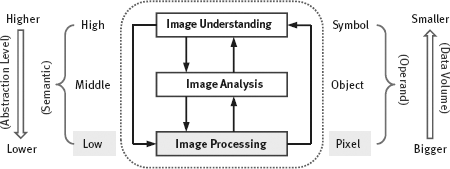
\includegraphics[width=0.5\textwidth, keepaspectratio]{08_Chapter01_fig1-4}
	\caption[]{\label{fig:sota:imageengineering} TODO Caption
	Reprinted from \textcite[][Chapter~1]{zhang2017imageprocessing}}
\end{figure}

\subsection{Object Detection}

TODO
edge detection, outline detection
foreground background mask from video image
background substraction

\subsection{Volume Estimation}

TODO
single view, multiview, depth sensors
estimation by pixel area
interpolation of depth information by combinding views
bounding / section box

\section{Elevator Control}
TODO

\subsection{System Components}
TODO

\subsection{System Classifications}
TODO
- by amount of elevators
- by type of sensory to haul the car
TODO how many elevators parallel
TODO additional travel information: how many people inside and outside, up / down / floor select inside / outside, everyone presses?, video? 
destination control system

\subsection{Passenger Flow Patterns}
TODO
TODO time of day eg. upstream, down stream, cross stream

\subsection{Control Strategies}

\subsection{Performance Criteria}
TODO
criteria: waiting time for passengers, riding time for passengers, capacity utilization, energy consumption, roundtriptime other times
ca 80\% oder auch 60-70\% maximal load on car, could be lower if objects in it
space vs wheight utilization
riding comfort in space and speed

\subsection{Simulational Optimization Approaches}
TODO
model building etc: here is a lot of research in the topic utilizing theoretical multivariable model optimization, simulational approaches and heuristical approaches in real world (refs?)

TODO
ISO standarts regarding lifts ISO4190 / EN 81

TODO
